%!TEX root = "../../../DA_GUI.tex"

%	--------------------------------------------------------
% 		Wissenschaftliche Analyse: Quests
%	--------------------------------------------------------

\subsection{Versuch zum Questsystem}
Bei unserem letzten Versuch wollten wir das Aufgabensystem testen, das bereits seit dem Sommer entwickelt wurde und in das wir eine beträchtliche Menge an Arbeit investiert hatten.

\subsubsection*{Gestellte Aufgaben}
Die Aufgaben wurden dieses Mal nicht in Form eines Übungszettels verteilt und von uns erklärt, sondern direkt vom Questsystem gestellt. Ziel des Versuches war, die Schüler der 1AHLES möglichst selbstständig arbeiten zu lassen und ihren Umgang mit dem Questsystem zu beobachten.

Alle Aufgaben bezogen sich auf das Thema \glqq{}Arrays\grqq{} und wurden --- zumindest in Grundzügen --- nach einem Arbeitsblatt von Herrn Pfoser erstellt.

Die erste Aufgabe war eine Übungsaufgabe, die wir zur Demonstration des Questsystems gemeinsam mit der Versuchsgruppe durchführten. Die Aufgaben waren:

\begin{enumerate}
\item \textbf{Einstiegsaufgabe:} Schreibe ein Programm, das die zahlen von 1 bis 10 in ein Array speichert und das Array ausgibt. 

\item \textbf{Array 10:} Schreibe ein Programm, das ein Array von 100 ganzen Zahlen anlegt, die sich als Produkt des Index mit 10 ergeben. Gib das Feld mit jeweils 10 Elementen Pro Zeile aus.

\item \textbf{Notendurchschnitt:} Eine Klasse mit 15 Schülerinnen und Schülern schreibt einen Test in FSST. Dabei kommen (logischerweise) 15 Noten zustande. Schreibe ein Programm, das den Durchschnitt der Noten berechnet. Die Noten sollen vom Eingabefeld eingelesen und in ein Array mit 15 Indizes gespeichert werden.

\item \textbf{Messwerte:} Erstelle ein C-Programm, das vom Benutzer bis zu 30 Messwerte (Gleitpunktzahlen) einlesen kann. Im Anschluss sollen jeweils der größte und der kleinste Wert und der arithmetische Mittelwert dieser Messreihe ausgegeben werden. Format der Ausgabe:
\begin{lstlisting}
Kleinste: 0.01
Groesste: 10.34
Durchschnitt: 4.42
\end{lstlisting}

\item \textbf{Fibonacci-Reihe:} Die Fibonacci-Reihe ist unendliche Folge von Zahlen, bei der die Summe zweier benachbarter Zahlen die unmittelbar folgende Zahl ergibt. Allgemein gilt:
\begin{equation}
f_n = f_{n-1} + f_{n-2}
\end{equation}
Allerdings muss es Anfangswerte geben. Deshalb gilt für die erste beiden Elemente:
\begin{equation}
f_1 = f_2 = 1
\end{equation}
Die ersten Elemente der Fibonacci-Reihe sind: 1, 1, 2, 3, 5, 8, 13, ... 

\item \textbf{Lottozahlen (Teil 1):} Simuliere eine Lotto-Ziehung. Die zufällig generierten Zahlen sollen in ein Array gespeichert und mit dem Befehl printIntArray ausgegeben werden (siehe Hinweise). Eine Zahl darf mehrmals vorkommen.

\item \textbf{Lottozahlen (Teil 2):} Simuliere eine Lotto-Ziehung. Die zufällig generierten Zahlen sollen in ein Array gespeichert und mit dem Befehl printIntArray ausgegeben werden (siehe Hinweise). Eine Zahl darf \textbf{nicht} mehrmals vorkommen.\\
\emph{Um diese Aufgabe zu bearbeiten, muss zuerst Aufgabe 1 gelöst werden}
\end{enumerate}
%TODO Bild von quest selecter?

\subsection*{Aufbau des Fragebogens}
Dieser Fragebogen war anders aufgebaut, als der Fragebogen für die ersten drei Versuche, da das Thema des Versuches das Questsystem war. Die Aufteilung der Fragen war dementsprechend ebenfalls etwas anders:
\begin{enumerate}
\item \textbf{Fragen 2 und 4:} Bedienung des Questsystems
\item \textbf{Frage 5:} Auftreten von Fehlern
\item \textbf{Fragen 3, 8 und 9:} Anwendung des Questsystems
\item \textbf{Frage 1: Verständlichkeit der Aufgaben}
\end{enumerate}

Bei zwei Freitextfragen wurden die Schüler wieder gebeten, ihre eigene Meinung und ihre Ideen für weitere Entwicklungsschritte einzubringen.

\subsubsection*{Ergebnisse: Fragen 2 und 4}

\emph{Frage 2: Ist das Questsystem (nicht die Entwicklungsumgebung selbst) gut zu bedienen? Sind die Bedienungsaktionen und -abläufe logisch und nachvollziehbar? \\
Frage 4: Wie gut sind die Entwicklungsumgebung und das Questsystem allgemein zu bedienen?}

\begin{figure}[h!]
\centering
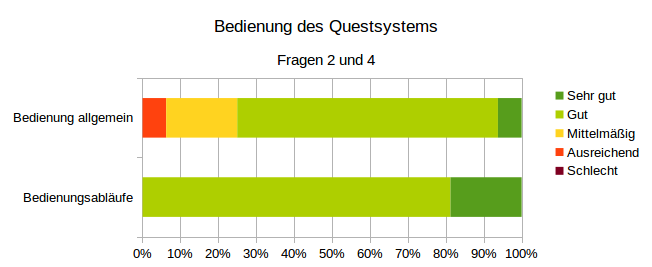
\includegraphics[width=0.95\textwidth]{./media/images/gui/trials/quest-f2-4.png}
\caption{Ergebnisse der Fragen 2 und 4}
\end{figure}

Das Konzept zur Bedienung des Questsystem wurde mehrmals überarbeitet und neu entworfen. Auf diese Weise wurde viel Aufwand in das Erscheinungsbild des Questsystems investiert. Die Antworten der Fragen 2 und 4 zeigen, dass sich dieser Aufwand gelohnt hat. Die Schüler hatten während des Versuches keine erkennbaren Probleme mit der Bedienung des Questsystems, dementsprechend sind die Antworten für diese Fragen sehr gut ausgefallen.
%TODO unterschied zwischen Frage 2 und 4 erklären?

\subsubsection*{Ergebnisse: Frage 5}

\emph{Frage 5: Gab es Probleme bei der Bedienung? Sind Fehler oder Bugs aufgetreten?}

\begin{figure}[h!]
\centering
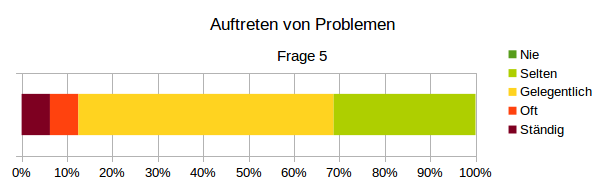
\includegraphics[width=0.95\textwidth]{./media/images/gui/trials/quest-f5.png}
\caption{Ergebnis der Frage 5}
\end{figure}

Die Schüler machten uns in dieser Frage zwar darauf Aufmerksam, dass das Questsystem noch nicht vollständig ausgereift ist, allerdings ist uns, wie oben erwähnt, aufgefallen, dass verhältnismäßig wenig Fehler, beziehungsweise wenig kritische Fehler (Abstürze, etc.) aufgetreten sind.

\subsubsection*{Ergebisse: Fragen 3, 8 und 9}

\emph{Frage 3: Ist es lustiger oder interessanter, Programmieraufgaben mit C Compact zu lösen?
Oder bearbeitest du lieber Aufgaben von einem Übungsblatt ab? \\
Frage 8: Stellt das Questsystem eine Verbesserung für den Unterricht dar? \\
Frage 9: Würdest du mit dem Questsystem ein bestimmtes Thema selbstständig erarbeiten können?}

\begin{figure}[h!]
\centering
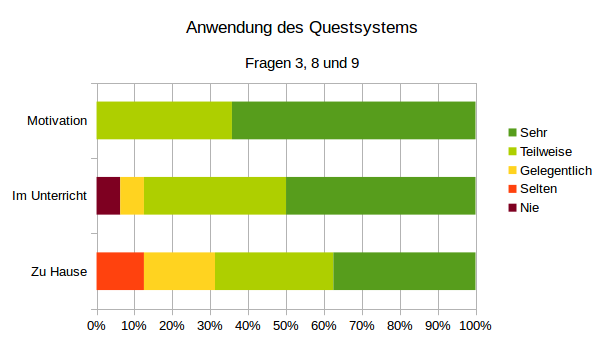
\includegraphics[width=0.95\textwidth]{./media/images/gui/trials/quest-f3-8-9.png}
\caption{Ergebnisse der Fragen 3, 8 und 9}
\label{fig:sci-quest-f3-8-9}
\end{figure}

Mit diesen Fragen wollten wir herausfinden, wo das Questsystem am besten zum Einsatz kommen kann. Wie sich in Frage 3 (in Abbildung \ref{fig:sci-quest-f3-8-9} oben) gezeigt hat, trägt das Questsystem wesentlich zur Motivation der Schüler bei. Es ist für die Schüler auf jeden Fall interessanter, Programmieraufgaben mit C Compact zu lösen. Diese Frage wurde von zwei Schülern nicht beantwortet, vermutlich, da die Frage nicht ganz eindeutig formuliert war.

Bei Frage 8 (mitte) gaben die meisten Schüler an, dass das Questsystem von C Compact eine Verbesserung für den Unterricht darstellt. Wir haben das Questsystem also tatsächlich so gestaltet, dass es in seinem Hauptzweck, dem Unterricht, Anwendung finden kann.

Allerdings sind die Antworten bei Frage 9 (unten) etwas schlechter ausgefallen.

\subsubsection*{Ergebnisse: Frage 1}

\emph{Frage 1: Waren die Aufgaben verständlich formuliert?}

\begin{figure}[h!]
\centering
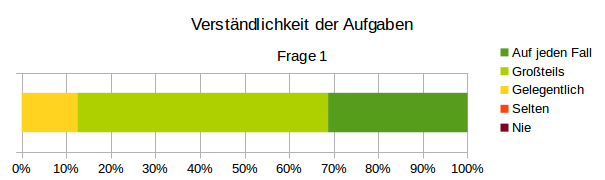
\includegraphics[width=0.95\textwidth]{./media/images/gui/trials/quest-f1.png}
\caption{Ergebnis der Frage 1}
\label{fig:sci-quest-f3-8-9}
\end{figure}

Mit dieser Aufgabe wollten wir herausfinden, ob wir die Aufgaben verständlich formuliert haben.

Es ist sehr schwierig, Aufgaben so zu formulieren, dass sie für jeden völlig verständlich sind. Im Zweifelsfall kann ein Schüler seinen Sitznachbarn oder den Lehrer fragen. Während des Versuches sind uns allerdings keine Probleme mit den Aufgaben an sich aufgefallen. Wir können die für den Versuche erstellten Aufgaben also durchaus als Beispiele (Demoaufgaben) verwenden.

\subsubsection*{Auswertung der Freitextfragen}

\emph{Frage 6: Welcher Bereich muss am dringendsten verbessert werden?\\
Frage 7: Was würdest du als nächstes hinzufügen?}

Bei Frage 6 wurden --- wie auch bei den anderen drei Versuchen --- unterschiedliche Ideen eingebracht. Die erwähnten Verbesserungsvorschläge reichten von leichten Optimierungen in der Benutzeroberfläche über Fehlermeldungen bis zu kleinen Verbesserungen im Questsystem. Allerdings wurde kein Vorschlag öfter als drei mal erwähnt, was darauf hindeutet, dass kein Problem besteht, das vielen Schülern wichtig ist.

Interessant ist, dass in Frage 7 der Vorschlag, mehr Quests und Tutorials zu erstellen, die meisten Erwähnungen zählt. Einige Schüler würden also offensichtlich gerne noch weitere Aufgaben lösen.

